\documentclass{article}

\textwidth=6.5in
\textheight=8.5in
\voffset=-54pt
\oddsidemargin=0in
\evensidemargin=0in
\setlength{\parskip}{8pt}
\setlength{\parindent}{0pt}

\usepackage{workbook}

\usepackage{handout}

\usepackage{exam}

\newcommand{\answerbox}[3][]{
    \fbox{\begin{minipage}[t][#2][c]{#3}
        #1
    \end{minipage}}
    }

\begin{document}

{\large \mbox{} \hfill \bf Name:\underline{\hspace{3in}}}\\[2pt]
{\mbox{} \hfill \it (Please write your name neatly in print.)}\\[12pt]
{\large \mbox{} \hfill \bf HUID:\underline{\hspace{3in}}}
 
\medskip
 
\noindent
{\large\bf
Exam 2 Practice 2\\
Math Mb Spring 2025}
\noindent


{\Large
\begin{center}\textbf{Directions---Please read carefully!} \end{center}}

This is a practice test. The same directions will appear on the actual exam, so read them carefully.

\hrulefill 


This exam is subject to the Harvard College Honor Code. No calculators or any other aids are permitted.  Please write as neatly as possible, as answers that can't be read can't be graded and thus can't receive credit. To receive full credit, you must show relevant working
and include units when appropriate. 

You have 120 minutes to complete this exam. 

You may ask for scratch paper if you need additional space to write, but it will not be scanned or graded. Make sure to include all relevant working in this exam booklet in the space provided for each question.

\begin{center}\textbf{Good luck!}\end{center}


\vfill

\centering{
\emph{As a member of Harvard College, I pledge that I will not give or receive assistance on this exam.}}
\vspace{0.3in}

{\large \mbox{} \hfill \bf Signature:\underline{\hspace{3in}}}
\thispagestyle{empty}

\newpage

\begin{enumerate}
\item \label{arctan-ln-graph}

  In this problem, you'll look at $\displaystyle f(x) = \arctan x + \ln
  \left( \frac{x^2 + 3}{x^2 + 1} \right)$.
  \begin{enumerate}
  \item \label{arctan-ln-graph-increasing}
    \begin{problem}[\vfill\vfill]
      For what values of $x$ is $f(x)$ increasing?
    \end{problem}

    \begin{solution}
      \ideas{To answer this, let's make a sign chart for $f'$, since we
        know that the sign of $f'$ tells us whether $f$ is increasing or
        decreasing.}

      First, we'll find the critical points, where $f'(x) = 0$.  Let's use
      log rules to simplify $f(x)$ before we differentiate:
      \begin{align*}
        f(x) &= \arctan x + \ln (x^2 + 3) - \ln (x^2 + 1) \\
        \intertext{Now, differentiate and simplify:}
        f'(x) &= \frac{1}{x^2 + 1} + \frac{1}{x^2 + 3} \cdot 2x -
        \frac{1}{x^2 + 1} \cdot 2x \\
        &= \frac{1 - 2x}{x^2 + 1} + \frac{2x}{x^2 + 3} \\
        &= \frac{(1 - 2x)(x^2 + 3) + (2x) (x^2 + 1)}{(x^2 + 1)(x^2 + 3)}
        \\
        &= \frac{x^2 + 3 - 2x^3 - 6x + 2x^3 + 2x}{(x^2 + 1)(x^2 + 3)} \\
        &= \frac{x^2 - 4x + 3}{(x^2 + 1)(x^2 + 3)} \\
        &= \frac{(x - 1)(x - 3)}{(x^2 + 1)(x^2 + 3)}
      \end{align*}
      Now, we'll solve $f'(x) = 0$:
      \begin{align*}
        \frac{(x - 1)(x - 3)}{(x^2 + 1)(x^2 + 3)} &= 0 \\
        (x - 1)(x - 3) &= 0 \\
        x &= 1, 3
      \end{align*}
      Now, we can make a sign chart for $f'$:
      \begin{center}
        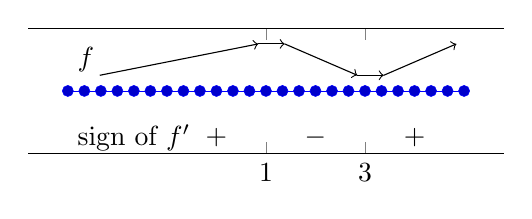
\begin{tikzpicture}
          \begin{axis}[axis y line=none, x axis line style={-}, xtick={1., 3.}, xticklabels={$1$, $3$}, ymin=-2, ymax=2, height=1.25in, width=3in]
            \addplot+[domain=-3.:5., very thin]{0};
            \draw (axis cs: -3., -1.5) node[right] {sign of $f'$};
            \draw (axis cs: -3., 1) node[right] {$f$};
            \draw (axis cs: 0., -1.5) node{$+$};
            \draw[->, xshift=2pt] (axis cs: -2.46667, 0.5) -- (axis cs: 0.733333, 1.5);
            \draw (axis cs: 2., -1.5) node{$-$};
            \draw[->, xshift=2pt] (axis cs: 1.26667, 1.5) -- (axis cs: 2.73333, 0.5);
            \draw (axis cs: 4., -1.5) node{$+$};
            \draw[->, xshift=2pt] (axis cs: 3.26667, 0.5) -- (axis cs: 4.73333, 1.5);
            \draw[->, xshift=2pt] (axis cs: 0.733333, 1.5) -- (axis cs: 1.26667, 1.5);
            \draw[->, xshift=2pt] (axis cs: 2.73333, 0.5) -- (axis cs: 3.26667, 0.5);
          \end{axis}
        \end{tikzpicture}
      \end{center}
      So, $f(x)$ is increasing on \fbox{$(-\infty, 1)$ and $(3,
        \infty)$}. 
    \end{solution}

  \item \label{arctan-ln-graph-limit-to-inf}
    \begin{problem}[\vfill]
      What is $\displaystyle \lim_{x \to \infty} f(x)$?  (\emph{Hint:}
      First find $\displaystyle \lim_{x \to \infty} \frac{x^2 + 3}{x^2 +
        1}$.)
    \end{problem}

    \begin{solution}
      Following the hint, let's first evaluate $\displaystyle \lim_{x \to
        \infty} \frac{x^2 + 3}{x^2 + 1}$.  This is an
      $\frac{\infty}{\infty}$ limit, and we can use relative growth rates
      to help.\footnote{You could also use L'H\^opital's Rule.}  In the
      sum $x^2 + 3$, $x^2$ is the faster growing term; in the sum $x^2 +
      1$, $x^2$ is the faster growing term.  So,
      \[ \lim_{x \to \infty} \frac{x^2 + 3}{x^2 + 1} = \lim_{x \to \infty}
      \frac{x^2}{x^2} = 1.\]
      So,
      \begin{align*}
        \lim_{x \to \infty} \left[ \arctan x + \ln \left( \frac{x^2 +
              3}{x^2 + 1} \right) \right] &= \left( \lim_{x \to \infty}
          \arctan x \right) + \ln 1 \\ 
        &= \frac{\pi}{2} + 0 \\
        &= \boxed{\frac{\pi}{2}}
      \end{align*}
    \end{solution}

  \item \label{arctan-ln-graph-limit-to-minus-inf}
    \begin{problem}[\vfill\newpage]
      What is $\displaystyle \lim_{x \to -\infty} f(x)$?
    \end{problem}

    \begin{solution}
      Using the same idea as in the previous part, we first evaluate
      $\displaystyle \lim_{x \to -\infty} \frac{x^2 + 3}{x^2 + 1}$:
      \[ \lim_{x \to -\infty} \frac{x^2 + 3}{x^2 + 1} = \lim_{x \to
        -\infty} \frac{x^2}{x^2} = 1.\]
      So,
      \begin{align*}
        \lim_{x \to -\infty} \left[ \arctan x + \ln \left( \frac{x^2 +
              3}{x^2 + 1} \right) \right] &= \left( \lim_{x \to -\infty}
          \arctan x \right) + \ln 1 \\ 
        &= - \frac{\pi}{2} + 0 \\
        &= \boxed{- \frac{\pi}{2}}
      \end{align*}
    \end{solution}

  \item
    \begin{problem}[\vfill]
      Does $f(x)$ have an absolute maximum?  If so, at what $x$-value(s)
      does it occur?  (\emph{Hint:} $\ln 2 \approx 0.69$.)
    \end{problem}

    \begin{solution}
      From our sign chart in \ref{arctan-ln-graph-increasing}, we see that
      $f(x)$ has a \textbf{local} maximum at $x = 1$, but it is not clear
      from the sign chart whether this is an absolute maximum, since
      $f(x)$ is increasing for $x > 3$.  So, we should compare $f(1)$ to
      $\displaystyle \lim_{x \to \infty} f(x)$.  We already calculated in
      \ref{arctan-ln-graph-limit-to-inf} that $\displaystyle \lim_{x \to
        \infty} f(x) = \frac{\pi}{2}$.  On the other hand, $f(1) = \arctan
      1 + \ln 2 = \frac{\pi}{4} + \ln 2 \approx \frac{\pi}{4} + 0.69$.  We
      are wondering how this compares to $\displaystyle \lim_{x \to
        \infty} f(x) = \frac{\pi}{2}$; that is, we want to know:
      \begin{align*}
        \frac{\pi}{4} + \ln 2 & \stackrel{?}{>} \frac{\pi}{2} \\
        \intertext{Subtracting $\frac{\pi}{4}$ from both sides,}
        \ln 2 & \stackrel{?}{>} \frac{\pi}{4} 
      \end{align*}
      The hint tells us that $\ln 2 \approx 0.69$, while $\pi \approx
      3.14$, so $\frac{\pi}{4} > \frac{3}{4} = 0.75$.  Therefore, the
      right side is actually bigger, so $\displaystyle \lim_{x \to \infty}
      f(x) > f(1)$.  This means that
      \begin{center}
        \fbox{$f(x)$ does not have an absolute maximum on $(-\infty,
          \infty)$.}
      \end{center}
    \end{solution}

  \item
    \begin{problem}[\vfill]
      Does $f(x)$ have an absolute minimum?  If so, at what $x$-value(s)
      does it occur?
    \end{problem}

    \begin{solution}
      From our sign chart in \ref{arctan-ln-graph-increasing}, we see that
      $f(x)$ has a \textbf{local} minimum at $x = 3$, but it is not clear
      from the sign chart whether this is an absolute minimum, since
      $f(x)$ is increasing for $x < 1$.  So, we should compare $f(3)$ to
      $\displaystyle \lim_{x \to -\infty} f(x)$.  We already calculated in
      \ref{arctan-ln-graph-limit-to-minus-inf} that $\displaystyle \lim_{x
        \to -\infty} f(x) = - \frac{\pi}{2}$.  On the other hand, $f(3) =
      \arctan 3 + \ln \frac{6}{5}$, which is definitely positive.  So,
      $f(3)$ is higher than $\displaystyle \lim_{x \to -\infty} f(x)$,
      which means that $f$ \fbox{does not have an absolute minimum on
        $(-\infty, \infty)$}.
    \end{solution}

  \item
    \begin{problem}[\vfill\vfill\newpage]
      Sketch a rough graph of $f(x)$.  Label all asymptotes clearly.
      (\emph{Note:} Your graph does \textbf{not} need to accurately
      indicate concavity, but it should incorporate what you found in the
      previous parts.)
    \end{problem}

    \begin{solution}
      \begin{center}
        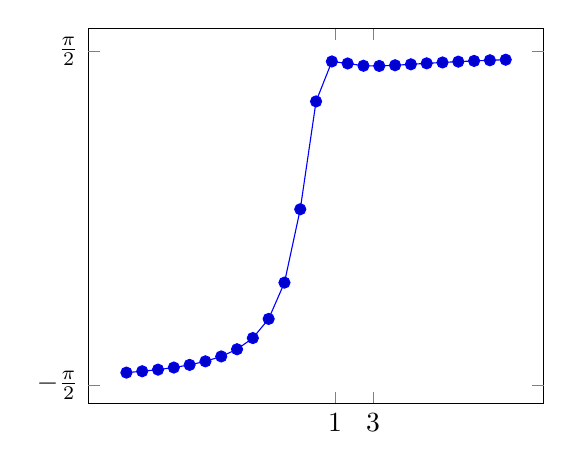
\begin{tikzpicture}
          \begin{axis}[extra y ticks={-1.57, 1.57}, extra y tick
            labels={$-\frac{\pi}{2}$, $\frac{\pi}{2}$}, xtick={1, 3},
            ytick=\empty, height=2.5in]
            \addplot+[domain=-10:10] { rad(atan(x)) + ln(x^2 + 3) - ln(x^2
              + 1)}; 
          \end{axis}
        \end{tikzpicture}
      \end{center}
    \end{solution}

    \begin{grading}
      The key features we're looking for are that it agrees with the
      previous parts.  That is:
      \begin{itemize}
      \item The graph increases on $(-\infty, 1)$, decreases on $(1, 3)$,
        and increases on $(3, \infty)$.
      \item $\displaystyle \lim_{x \to \infty} f(x) = \frac{\pi}{2}$ and
        $\displaystyle \lim_{x \to -\infty} f(x) = - \frac{\pi}{2}$.
      \item The local maximum at $x = 1$ is below $y = \frac{\pi}{2}$, and
        the local minimum at $x = 3$ is above $y = - \frac{\pi}{2}$.
      \end{itemize}
    \end{grading}

  \end{enumerate}
  
  \pspace{\newpage}



\item \label{spring2004-xb-midterm2-7} 



  Let $p(t)$ be the rate of growth (in meters per year) of a particular
  pine tree at time $t$, where $t$ is measured in years.  Let $f(t)$ be
  the rate of growth (in meters per year) of a particular fir tree.  The
  graphs of $p(t)$ and $f(t)$ are given below.  Assume that the two
  trees were the same height $H$ at $t=0$.

  \begin{center}
    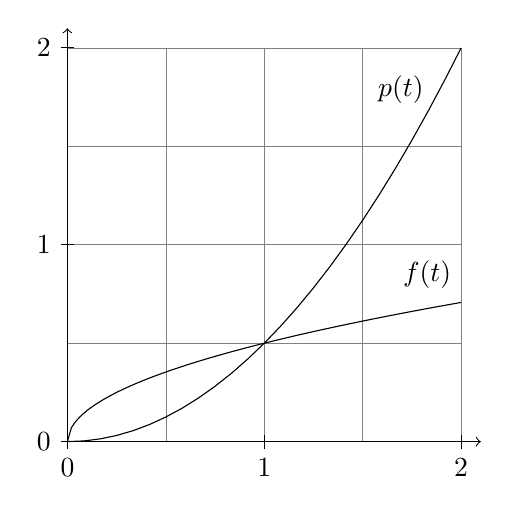
\begin{tikzpicture}[scale=2.5]
      \def\p{\x,{\x*\x/2}}
      \def\f{\x,{1/2*sqrt(\x)}}

      % grid
      \draw[very thin, color=gray] (0,0) grid[step=0.5] (2, 2);

      % axes 
      \draw[->] (0,0) -- (2.1,0);
      \draw[->] (0,0) -- (0,2.1);
      \foreach \x in {0, 1, 2}
      \draw (\x,-1pt) node[below] {$\x$} -- (\x,1pt);
      \foreach \y in {0, 1, 2}
      \draw (-1pt,\y) node[left] {$\y$} -- (1pt,\y);

      % the curves
      \draw[domain=0:2, samples=100] plot (\f) node[left, yshift=1em] {$f(t)$};
      \draw[domain=0:2] plot (\p) node[left, xshift=-1em, yshift=-1.5em] {$p(t)$};
    \end{tikzpicture}
  \end{center}

  \begin{enumerate}
  \item
    \begin{problem}[\vfill]
      Write an expression for the height of the pine tree after six
      months.  Your expression should involve a definite integral.  
    \end{problem}

    \begin{solution}
      The pine tree's 
      height at time $0$  was $H$.  Between $t = 0$ and $t = 0.5$ (six
      months), the tree grew by $\displaystyle \int_0^{0.5} p(t)\,dt$.  So,
      the pine tree's height after 6 months is $\boxed{H + \int_0^{0.5}
        p(t)\,dt}$. 
    \end{solution}

  \item
    \begin{problem}[\vfill]
      Which tree is taller after 1 year?  Please explain. 
    \end{problem}

    \begin{solution}
      The \fbox{fir}, because $f(t) > p(t)$ during the first year (this
      means that the fir is growing faster than the pine throughout the
      first year; since they started out the same height, the fir must be
      taller by the end of the year).
    \end{solution}

  \item
    \begin{problem}[\vfill]
      Which tree is taller after 2 years?  Please explain. 
    \end{problem}

    \begin{solution}
      The \fbox{pine}.  The fir's height at the end of 2 years is $H +
      \displaystyle \int_0^2 f(t)\,dt$, while the pine's height at the end
      of 2 years is $H + \displaystyle \int_0^2 p(t)\,dt$.  We can see from
      the graphs that $\displaystyle \int_0^2 p(t)\,dt > \int_0^2 h(t)\,dt$.
    \end{solution}

  \item
    \begin{problem}[\vfill]
      At approximately what time(s) are the trees growing at the same
      rate?  Justify your answer.
    \end{problem}

    \begin{solution}
      Since these graphs are rate graphs, this question is simply asking
      when the graphs intersect.  This happens at \fbox{$t=0$ and $t=1$}.
    \end{solution}

  \item
    \begin{problem}[\vfill\newpage]
      At approximately what time(s) after $t = 0$ are the trees the same
      height?  Justify your answer.
    \end{problem}

    \begin{solution}
      At time $T$, the fir has height $\displaystyle H + \int_0^T
      f(t)\,dt$, while the pine has height $\displaystyle H + \int_0^T
      p(t)\,dt$.  These will be equal if $\displaystyle \int_0^T f(t)\,dt =
      \int_0^T p(t)\,dt$.  Graphically, we are looking for the time $T$
      such that the areas under $f(t)$ and $p(t)$ from $t = 0$ to $t = T$
      are the same (i.e., when the red and blue regions below are equal).

      \begin{tikzpicture}[scale=2.5]
        \def\p{\x,{\x*\x/2}}
        \def\f{\x,{1/2*sqrt(\x)}}
        \def\T{4^(1/3)}

        % grid
        \draw[very thin, color=gray] (0,0) grid[step=0.5] (2, 2);

        % axes 
        \draw[->] (0,0) -- (2.1,0);
        \draw[->] (0,0) -- (0,2.1);
        \foreach \x in {0, 1, 2}
        \draw (\x,-1pt) node[below] {$\x$} -- (\x,1pt);
        \foreach \y in {0, 1, 2}
        \draw (-1pt,\y) node[left] {$\y$} -- (1pt,\y);

        % shade area under curve
        \fill [pattern color=red,pattern=north east lines] (0, 0) --
        plot[domain=0:\T] (\f) -- ({\T},0) -- cycle;
        \fill [pattern color=blue,pattern=north west lines] (0, 0) -- plot[domain=0:\T] (\p) -- ({\T},0) -- cycle;

        % the curves
        \draw[domain=0:2, samples=100] plot (\f) node[left, yshift=1em] {$f(t)$};
        \draw[domain=0:2] plot (\p) node[left, xshift=-1em, yshift=-1.5em] {$p(t)$};

        % ticks
        \draw ({\T}, 1pt) -- ({\T}, -1pt) node[below] {$T$};
      \end{tikzpicture}

      Although we can't find this value of $T$ exactly, it looks like it
      happens at about $T \approx  \boxed{1.6}$.
    \end{solution}

  \end{enumerate}

\item 
  \label{spring2008-midterm2-4-expanded}



  \begin{enumerate}
  \item 
    \begin{problem}[\vfill]
      Evaluate $\displaystyle \lim_{x\rightarrow 1^-}\frac{\arcsin (x)
        -\pi/2}{\sqrt{1-x^2}}.$
    \end{problem}

    \begin{solution}
      As $x \to 1^-$, $\arcsin(x) - \frac{\pi}{2} \to \arcsin (1) -
      \frac{\pi}{2} = \frac{\pi}{2} - \frac{\pi}{2} = 0$ and $\sqrt{1 -
        x^2} \to \sqrt{1 - 1^2} = 0$.  Therefore, this limit is of the
      indeterminate form $\frac{0}{0}$, and we'll use L'H\^opital's Rule: 
      \begin{align*}
        \lim_{x \to 1^-} \frac{\arcsin (x) - \frac{\pi}{2}}{(1 -
          x^2)^{1/2}} & \stackrel{\text{L'H}}{=} \lim_{x \to 1^-}
        \frac{\frac{1}{\sqrt{1
              - x^2}}}{ \frac{1}{2} (1 - x^2)^{-1/2} (-2x)} \\
        &= \lim_{x \to 1^-} \frac{\frac{1}{\sqrt{1
              - x^2}}}{ -x (1 - x^2)^{-1/2}} \\
        &= \lim_{x \to 1^-} \frac{1}{-x} \\
        &= \boxed{-1}
      \end{align*}
    \end{solution}

  \item
    \begin{problem}[\vfill]
      Evaluate $\displaystyle \lim_{x\rightarrow 0}\frac{\arcsin (x)
        -\pi/2}{\sqrt{1-x^2}}.$
    \end{problem}

    \begin{solution}
      As $x \to 0$, $\arcsin(x) - \frac{\pi}{2} \to \arcsin(0) -
      \frac{\pi}{2} = - \frac{\pi}{2}$ and $\sqrt{1 - x^2} \to \sqrt{1 -
        0^2} = 1$.  So, $\displaystyle \lim_{x \to 0} \frac{\arcsin (x)
        -\pi/2}{\sqrt{1-x^2}} = \boxed{- \frac{\pi}{2}}$.       
    \end{solution}

  \item
    \begin{problem}[\vfill]
      Evaluate $\displaystyle \lim_{x\rightarrow -1^+}\frac{\arcsin (x)
        -\pi/2}{\sqrt{1-x^2}}.$
    \end{problem}

    \begin{solution}
      As $x \to -1^+$, $\arcsin(x) - \frac{\pi}{2} \to \arcsin (-1) -
      \frac{\pi}{2} = - \frac{\pi}{2} - \frac{\pi}{2} = - \pi$ and
      $\sqrt{1 - x^2} \to \sqrt{1 - (-1)^2} = 0$.  In this situation, we
      must think about the sign of the denominator.  The denominator is
      always positive, so when $x$ is slightly bigger than $-1$,
      $\displaystyle \frac{\arcsin (x) -\pi/2}{\sqrt{1-x^2}}$ involves
      dividing a number close to $-\pi$ by a tiny positive number, which
      gives a very negative result.  Therefore, $\displaystyle \lim_{x \to
        -1^+} \frac{\arcsin (x) -\pi/2}{\sqrt{1-x^2}} = \boxed{-\infty}$.
    \end{solution}



  \end{enumerate}

\item \label{spring2011-mb-final-7}   



  \begin{enumerate}
  \item 
    \begin{problem}[\vfill]
      On the left set of axes below, sketch $y = \tan x$ on the interval
      $[-4, 4]$.  Clearly indicate all asymptotes.
    \end{problem}

    \begin{problemonly}
      \axes[xtick={-4, -3, ..., 4}, ytick={-4, -3, ..., 4}, xmin=-4,
      ymin=-4, xmax=4.5, ymax=4.5, width=3.25in, height=3.25in]
      \hspace{0.25in}      
      \axes[xtick={-8, -6, ..., 8}, minor xtick={-7, -5, ..., 7},
      ytick=\empty, xmin=-8, xmax=8.5, width=3.25in, height=3.25in]      
    \end{problemonly}

    \begin{solution}
      The asymptotes of $\tan x$ are at $\pm \frac{\pi}{2},
      \pm \frac{3 \pi}{2}, \ldots$. (Since $\pi$ is a bit bigger than 3,
      $\frac{\pi}{2}$ is a bit bigger than $1.5$.)  The zeros are at $0,
      \pm \pi, \pm 2 \pi, \ldots$. 
      \begin{center}
        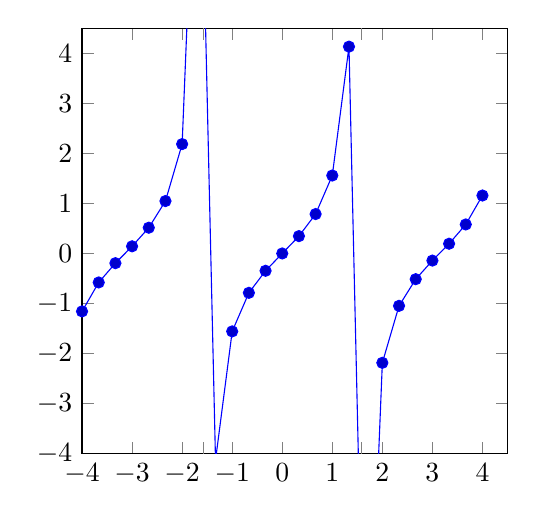
\begin{tikzpicture}
          \begin{axis}[xtick={-4, -3, ..., 4}, ytick={-4, -3, ..., 4},
            xmin=-4, ymin=-4, xmax=4.5, ymax=4.5, width=2.75in,
            height=2.75in, extra x ticks={-4.71239, -1.5708, 1.5708,
              4.71239}, extra x tick labels={}]
            \addplot+[domain=-4:4, restrict y to
            domain=-20:20]{tan(deg(x))};            
          \end{axis}
        \end{tikzpicture}
      \end{center}
    \end{solution}

  \item
    \begin{problem}[\vfill]
      Sketch $y =  \arctan x$ on the right set of axes above.  Label any
      important values on the $y$-axis. 
    \end{problem}

    \begin{solution}
      \begin{center}
        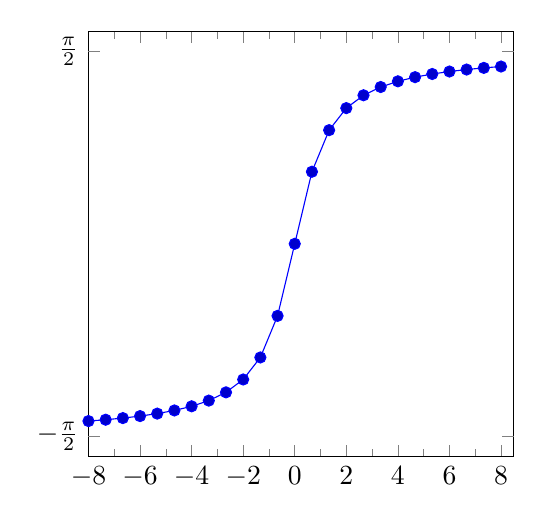
\begin{tikzpicture}
          \begin{axis}[xtick={-8, -6, ..., 8}, minor xtick={-7, -5, ...,
              7}, ytick=\empty, xmin=-8, xmax=8.5, width=2.75in,
            height=2.75in, extra y ticks={-1.5708, 1.5708}, extra y tick
            labels={$-\frac{\pi}{2}$, $\frac{\pi}{2}$}]
            \addplot+[domain=-8:8] {rad(atan(x))};
          \end{axis}
        \end{tikzpicture}
      \end{center}      
    \end{solution}

  \item \label{spring2011-final-7-arctan-region}
    \begin{problem}[\vfill]
      On your graph of $y = \arctan x$, lightly shade a region whose area
      is $\displaystyle \int_3^{7} \arctan x\,dx$.
    \end{problem}

    \begin{solution}
      \begin{center}
        \begin{tikzpicture}
          \begin{axis}[xtick={-8, -6, ..., 8}, minor xtick={-7, -5, ...,
              7}, ytick=\empty, xmin=-8, xmax=8.5, width=2.75in,
            height=2.75in, extra y ticks={-1.5708, 1.5708}, extra y tick
            labels={$-\frac{\pi}{2}$, $\frac{\pi}{2}$}]
            \addplot+[domain=3:7, plusarea] {rad(atan(x))} \closedcycle;
            \addplot+[domain=-8:8, black] {rad(atan(x))};
          \end{axis}
        \end{tikzpicture}
      \end{center}      
    \end{solution}

  \item \label{spring2011-final-7-arctan-L4} 
    \begin{problem}[\vfill\vfill\newpage]
      Draw a pictorial representation of $L_4$, the left hand sum with 4
      rectangles that approximates the integral $\displaystyle \int_3^{7}
      \arctan x\,dx$.  Write out an expression for $L_4$ (you need not
      simplify). 
    \end{problem}

    \begin{solution}
      \begin{center}
        \begin{tikzpicture}[declare function={f(\x)=rad(atan(\x));}]
          \begin{axis}[xtick={-8, -6, ..., 8}, minor xtick={-7, -5, ...,
              7}, ytick=\empty, xmin=-8, xmax=8.5, width=2.75in,
            height=2.75in, extra y ticks={-1.5708, 1.5708}, extra y tick
            labels={$-\frac{\pi}{2}$, $\frac{\pi}{2}$}]
            \addplot+[ybar interval, plusarea] coordinates { (3, {f(3)})
              (4, {f(4)}) (5, {f(5)}) (6, {f(6)}) (7, {f(6)}) }; 
            \addplot+[domain=-8:8, black] {f(x)};
          \end{axis}
        \end{tikzpicture}
      \end{center}
      Each rectangle in this sum has width 1, so $L_4 = (\arctan 3) (1) +
      (\arctan 4) (1) + (\arctan 5) (1) + (\arctan 6) (1)$.
    \end{solution}

  \item Put the following quantities in ascending order, from smallest to
    largest.  (You can do this using the letters corresponding to your
    choices.  Use ``$<$'' or ``='' signs.)
    \begin{enumerate}[label=\Alph*.]
    \item $\displaystyle \int_3^{7} \arctan x\,dx$

    \item $\displaystyle \arctan 3 + \arctan 4 + \arctan 5 + \arctan 6$

    \item $\displaystyle \arctan 4 + \arctan 5 + \arctan 6 + \arctan 7$

    \item $\displaystyle \int_{-3}^3 \arctan x\,dx$
    \item $\displaystyle \int_{-1}^0 \arctan x\,dx$  
    \item $\displaystyle \int_{-3}^1 \arctan x\,dx$  
    \item $\displaystyle \int_{1}^0 \arctan x\,dx$     
    \end{enumerate}

    \pspace{\vfill}

    \textbf{From smallest to largest:} $\fitb{3.5in}{F < E = G < D < B < A <
      C}$

    \pspace{\newpage}

    \begin{solution}
      Let's look at these quantities one by one. 
      \begin{enumerate}[label=\Alph*.]
      \item $\displaystyle \int_3^{7} \arctan x\,dx$: This is the area we
        shaded in \ref{spring2011-final-7-arctan-region}. 

      \item $\displaystyle \arctan 3 + \arctan 4 + \arctan 5 + \arctan 6$:
        This is $L_4$, which we sketched in
        \ref{spring2011-final-7-arctan-L4}.  From that picture, we can see
        that this is slightly smaller than A.

      \item $\displaystyle \arctan 4 + \arctan 5 + \arctan 6 + \arctan 7$:
        This is $R_4$, which is slightly bigger than A.  (So, so far we have
        the ordering $B < A < C$.)

      \item $\displaystyle \int_{-3}^3 \arctan x\,dx$: This is the signed
        area shaded here:
        \begin{center}
          \begin{tikzpicture}[declare function={f(\x)=rad(atan(\x));}]
            \begin{axis}[xtick={-8, -6, ..., 8}, minor xtick={-7, -5, ...,
                7}, ytick=\empty, xmin=-8, xmax=8.5, width=2.5in,
              height=2in, extra y ticks={-1.5708, 1.5708}, extra y tick
              labels={$-\frac{\pi}{2}$, $\frac{\pi}{2}$}]
              \addplot+[domain=-3:0, minusarea] {f(x)} \closedcycle;
              \addplot+[domain=0:3, plusarea] {f(x)} \closedcycle;
              \addplot+[domain=-8:8, black] {f(x)};
            \end{axis}
          \end{tikzpicture}
        \end{center}
        By symmetry, this is equal to 0.  The previous quantities were all
        positive, so we have $D < B < A < C$.

      \item $\displaystyle \int_{-1}^0 \arctan x\,dx$: This is the signed
        area shaded here:
        \begin{center}
          \begin{tikzpicture}[declare function={f(\x)=rad(atan(\x));}]
            \begin{axis}[xtick={-8, -6, ..., 8}, minor xtick={-7, -5, ...,
                7}, ytick=\empty, xmin=-8, xmax=8.5, width=2.5in,
              height=2in, extra y ticks={-1.5708, 1.5708}, extra y tick
              labels={$-\frac{\pi}{2}$, $\frac{\pi}{2}$}]
              \addplot+[domain=-1:0, minusarea] {f(x)} \closedcycle;
              \addplot+[domain=-8:8, black] {f(x)};
            \end{axis}
          \end{tikzpicture}
        \end{center}
        We can see that this is negative.

      \item $\displaystyle \int_{-3}^1 \arctan x\,dx$: This is the signed
        area shaded here:
        \begin{center}
          \begin{tikzpicture}[declare function={f(\x)=rad(atan(\x));}]
            \begin{axis}[xtick={-8, -6, ..., 8}, minor xtick={-7, -5, ...,
                7}, ytick=\empty, xmin=-8, xmax=8.5, width=2.5in,
              height=2in, extra y ticks={-1.5708, 1.5708}, extra y tick
              labels={$-\frac{\pi}{2}$, $\frac{\pi}{2}$}]
              \addplot+[domain=-3:0, minusarea] {f(x)} \closedcycle;
              \addplot+[domain=0:1, plusarea] {f(x)} \closedcycle;
              \addplot+[domain=-8:8, black] {f(x)};
            \end{axis}
          \end{tikzpicture}
        \end{center}
        By symmetry, we can see that the signed area from $-1$ to $0$
        cancels the signed area from 0 to 1, so another way of visualizing
        $\displaystyle \int_{-3}^1 \arctan x\,dx$ is this:
        \begin{center}
          \begin{tikzpicture}[declare function={f(\x)=rad(atan(\x));}]
            \begin{axis}[xtick={-8, -6, ..., 8}, minor xtick={-7, -5, ...,
                7}, ytick=\empty, xmin=-8, xmax=8.5, width=2.5in,
              height=2in, extra y ticks={-1.5708, 1.5708}, extra y tick
              labels={$-\frac{\pi}{2}$, $\frac{\pi}{2}$}]
              \addplot+[domain=-3:-1, minusarea] {f(x)} \closedcycle;
              \addplot+[domain=-8:8, black] {f(x)};
            \end{axis}
          \end{tikzpicture}
        \end{center}
        This is clearly more negative than E. 

      \item
        $\displaystyle \int_{1}^0 \arctan x\,dx$: This is equal to
        $\displaystyle - \int_0^1 \arctan x\,dx$, which is the negative of
        this area: 
        \begin{center}
          \begin{tikzpicture}[declare function={f(\x)=rad(atan(\x));}]
            \begin{axis}[xtick={-8, -6, ..., 8}, minor xtick={-7, -5, ...,
                7}, ytick=\empty, xmin=-8, xmax=8.5, width=2.5in,
              height=2in, extra y ticks={-1.5708, 1.5708}, extra y tick
              labels={$-\frac{\pi}{2}$, $\frac{\pi}{2}$}]
              \addplot+[domain=0:1, plusarea] {f(x)} \closedcycle;
              \addplot+[domain=-8:8, black] {f(x)};
            \end{axis}
          \end{tikzpicture}
        \end{center}
        This is equal to E.

      \end{enumerate}
      That gives a final ordering of $F < E = G < D < B < A < C$. 
    \end{solution}

    % \item It is unlikely that you know an antiderivative of $\arctan x$.  Suppose that you want to evaluate $\displaystyle \int_{0}^1 \arctan x\,dx$ exactly.  "There are several ways you can do it. Either find a way and explain it to us, or follow the suggestion below:

    %   Draw a new picture and lightly shade in the area corresponding to this integral. Now, by slicing with respect to $y$, rather than $x$, find the area. This must be exactly $\displaystyle \int_{0}^1 \arctan x\,dx$.

  \end{enumerate}

\item \label{spring2012-mb-midterm2-1}  % Rachel Epstein


  An investor buys some stock at time $t = 0$; time $t$ is measured in
  days.  The function $r(t)$, given by the graph below, gives the rate of
  change of the value of his stock in dollars per day.
  At time $t = 6$, the stock is worth \$75.

  \begin{center}
    \begin{tabular}{c}
    {\small $f(t) = $ rate of change of island's population} \\
      {\small (people per year)} \\
        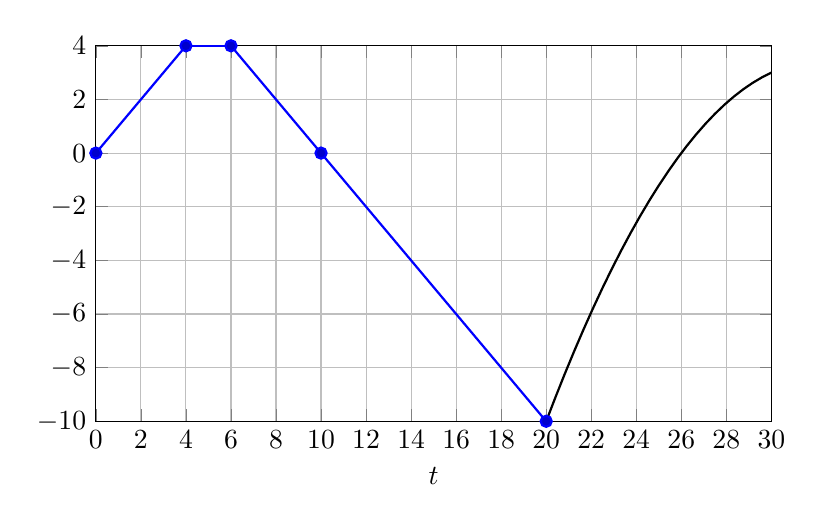
\begin{tikzpicture}
        \begin{axis}[grid=major, ymin=-10, ymax=4, xmin=0, xmax=30, xtick={0, 2, ..., 30}, ytick={-10, -8, ..., 4}, 
          xlabel=$t$,
          width=4in, height=2.5in] 
          \addplot+[sharp plot, thick] coordinates { (0, 0) (4, 4) (6, 4) (20, -10)
            (10, 0) };
          \addplot[thick, domain=20:30]{-11/120*x^2 + 353/60*x - 91};
        
        \end{axis}
      \end{tikzpicture}
        \end{tabular}
      \end{center}


  \begin{enumerate}
  \item
    \begin{problem}[\vfill]
      The investor sells the stock after 30 days, at time $t=30$.  Express
      his net gain/loss (from when the investor bought the stock, at time
      $t = 0$, to when he sold the stock, at time $t = 30$) as a definite
      integral.
    \end{problem}

    \begin{solution}
      The net change is $\boxed{ \int_0^{30} r(t)\,dt}$.
    \end{solution}

  \item
    \begin{problem}[\vfill]
      Overall (from when the investor bought the stock, at time $t = 0$,
      to when he sold the stock, at time $t = 30$), did the stock's value
      rise or fall?  Explain briefly.
    \end{problem}

    \begin{solution}
      The integral $\displaystyle \int_0^{30} r(t)\,dt$ can be visualized
      as the signed area under $r(t)$ from $t = 0$ to $t = 30$; we can see
      that this area is negative, so the stock's value \fbox{fell}. 
    \end{solution}

  \item
    \begin{problem}[\vfill]
      What is the value of the stock at time $t = 12$?  (Your answer should
      be a number; it should not include any integral signs.) 
    \end{problem}

    \begin{solution}
      We are told that the stock is worth \$75 at time $t = 6$.  From $t =
      6$ to $t = 12$, it changed by $\displaystyle \int_6^{12} r(t)\,dt$,
      so the price at $t = 12$ is $75 + \displaystyle \int_6^{12}
      r(t)\,dt$.  Since the problem asks for a number, we should evaluate
      this.  By interpreting $\displaystyle \int_6^{12} r(t)\,dt$ as
      signed area, we see that it's equal to $6$, so the value of the
      stock at time $t=12$ is $\$75 + \$6 = \boxed{\$81}$.
    \end{solution}

  \item \label{spring2012-mb-midterm2-1d}
    \begin{problem}[\vfill]
      At what time (between $0$ and $30$) was the stock worth the most?
      (No explanation is necessary.)
    \end{problem}

    \begin{solution}
      The stock's value increases when $r(t)$ is positive and decreases
      when $r(t)$ is negative.  Therefore, we can see the stock's value
      increases on $(0, 10)$, decreases on $(10, 26)$, and increases again
      on $(26, 30)$.  We can put that information in a diagram:
      \begin{center}
        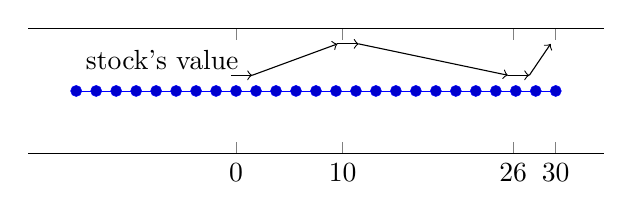
\begin{tikzpicture}
          \begin{axis}[axis y line=none, x axis line style={-}, xtick={0., 10., 26., 30.}, xticklabels={$0$, $10$, $26$, $30$}, ymin=-2, ymax=2, height=1.25in, width=3.5in]
            \addplot+[domain=-15.:30., very thin]{0};
            \draw (axis cs: -15., 1) node[right] {stock's value};
            \draw[->, xshift=2pt] (axis cs: -1, 0.5) -- (axis cs: 1, 0.5);
            \draw[->, xshift=2pt] (axis cs: 1, 0.5) -- (axis cs: 9., 1.5);
            \draw[->, xshift=2pt] (axis cs: 11., 1.5) -- (axis cs: 25., 0.5);
            \draw[->, xshift=2pt] (axis cs: 27., 0.5) -- (axis cs: 29., 1.5);
            \draw[->, xshift=2pt] (axis cs: 9., 1.5) -- (axis cs: 11., 1.5);
            \draw[->, xshift=2pt] (axis cs: 25., 0.5) -- (axis cs: 27., 0.5);
          \end{axis}
        \end{tikzpicture}
      \end{center}
      So, the stock is worth the most either at $t = 10$ or $t = 30$.  To
      compare these two, let's look at the net change in the stock's value
      from $t = 10$ to $t = 30$, which is $\displaystyle \int_{10}^{30}
      r(t)\,dt$.  We can see from the graph that this integral is
      negative, which means that the stock had a net loss in value from $t
      = 10$ to $t = 30$.  Therefore, the stock was worth the most at
      \fbox{$t = 10$}.
    \end{solution}

  \item
    \begin{problem}[\vfill\newpage]
      At what time (between $0$ and $30$) was the stock worth the least?
      (No explanation is necessary.)
    \end{problem}

    \begin{solution}
      From our diagram in \ref{spring2012-mb-midterm2-1d}, the stock is
      worth the least at either $t = 0$ or $t = 26$.  To compare these
      two, let's look at the net change in the stock's value from $t = 0$
      to $t = 26$, which is $\displaystyle \int_0^{26} r(t)\,dt$.  We can
      see from the graph that this integral is negative, so the stock had
      a net loss in value from $t = 0$ to $t = 26$. Therefore, the stock
      was worth the least at \fbox{$t=26$}.  
    \end{solution}
  \end{enumerate}

\item
  \label{spring2010-mb-midterm2-6}
  \label{integral-graphical-comparisons-1} 


  The graph of a function $f(x)$ defined on $[1, 10]$ is given below.

  {
    \newcommand{\graphinside}{%
      \addplot+[domain=1:4] {3.2657389299250745 - 0.32180828170540376*x + 0.07431133993842803*x^2 - 0.018241988158098566*x^3}; %
      \addplot+[domain=4:6] {-0.7791830417797501 + 2.331470848926667*x - 0.4936373134846165*x^2 + 0.021117135341046023*x^3}; %
      \addplot+[domain=6:7] {-150.10447902340712 + 74.49717175726747*x - 12.129357677718435*x^2 + 0.6471218744336391*x^3}; %
      \addplot+[domain=7:7.5] {-39.780564069511215 + 30.54257213567293*x - 6.340462242654196*x^2 + 0.3955253906992896*x^3}; %
      \addplot+[domain=7.5:8] {-3271.2493913984017 + 1254.293572394858*x - 160.37842209101555*x^2 + 6.838124660282293*x^3}; %
      \addplot+[domain=8:10] {-12.56107226311967 + 3.242771362944227*x - 0.2907326766310134*x^2 + 0.010206626296778737*x^3}; %
    }

    \begin{center}
      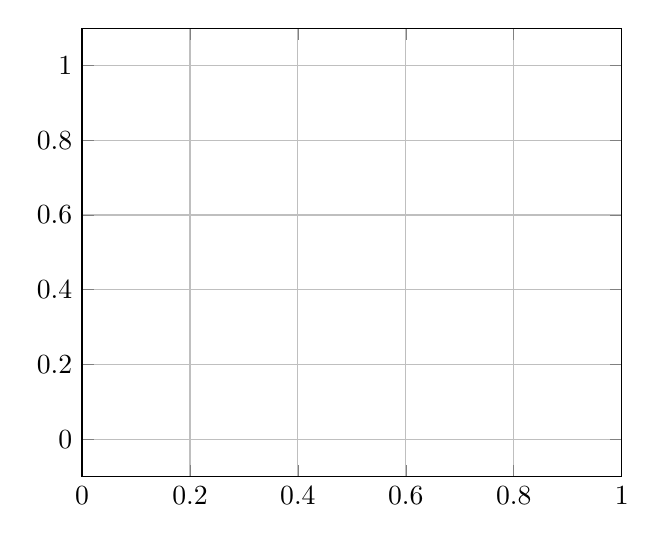
\begin{tikzpicture}
        \begin{axis}[cycle list=black, grid=major, xtick={1, 2, ..., 10},
          xmin=0, xmax=10.5]
          \graphinside
        \end{axis}
      \end{tikzpicture}
    \end{center}

    \begin{enumerate}
    \item
      \begin{problem}[\vfill]
        Approximate $\displaystyle \int_1^7 f(x)\,dx$ by computing $R_2$ and
        $L_2$.  Is each approximation an overestimate or an underestimate?
      \end{problem}

      \begin{solution}
        Graphically, $L_2$ and $R_2$ represent the signed areas of the
        following rectangles:
        \begin{center}
          \begin{tabular}{c c c}
            \begin{tikzpicture}
              \begin{axis}[cycle list=black, grid=major, xtick={1, 2, ..., 10},
                xmin=0, xmax=10.5, width=2.5in, ytick={-1, 0, ..., 3}]
                \graphinside
                \addplot[ybar interval, plusarea] coordinates
                {
                  (1, 2)
                  (4, 2)
                };
                \addplot[ybar interval, minusarea] coordinates 
                {
                  (4, -1)
                  (7, -1)
                };
              \end{axis}
            \end{tikzpicture}
            & \hspace{0.25in} &
            \begin{tikzpicture}
              \begin{axis}[cycle list=black, grid=major, xtick={1, 2, ..., 10},
                xmin=0, xmax=10.5, width=2.5in, ytick={-1, 0, ..., 3}]
                \graphinside
                \addplot[ybar interval, plusarea] coordinates
                {
                  (1, 3)
                  (4, 2)
                  (7, 2)
                };
              \end{axis}
            \end{tikzpicture}
            \\
            $R_2$ & & $L_2$
          \end{tabular}        
        \end{center}
        From this, we can see that $R_2 = f(4) \cdot 3 + f(7) \cdot 3 = (2)
        (3) + (-1) 3 = 3$ and $L_2 = f(1) \cdot 3 + f(4) \cdot 3 = (3) 3 +
        (2) 3 = 15$.

        We can also see from the pictures that $R_2$ is an underestimate for
        $\displaystyle \int_1^7 f(t)\,dt$, and $L_2$ is an overestimate (this
        happens because $f$ is decreasing on $[1, 7]$).

      \end{solution}

    \item 
      \begin{problem}[\vfill]
        Suppose we approximate $\displaystyle \int_1^4 f(x)\,dx$ using
        several left-hand and right-hand sums $L_n$ and $R_n$.  Put the
        following expressions in increasing order, with ``$<$'' or ``$=$''
        signs between them:
        \[ \int_1^4 f(x)\,dx \qquad L_4 \qquad L_{12} \qquad R_4 \qquad
        R_{12} \qquad \lim_{n \to \infty} L_n \qquad \lim_{n \to \infty}
        R_n \]
      \end{problem}

      \begin{solution}
        First, $\displaystyle \lim_{n \to \infty} L_n$ and $\displaystyle
        \lim_{n \to \infty} R_n$ are both equal to $\displaystyle \int_1^4
        f(x)\,dx$ by the definition of the definite integral.

        Since $f$ is decreasing from 1 to 4, any right-hand sum is an
        underestimate for $\displaystyle \int_1^4 f(x)\,dx$, and any
        left-hand sum is an overestimate.  Also, using more rectangles gives
        better approximations in this case, so $R_{12}$ and $L_{12}$ are
        closer to the actual integral than $R_4$ and $L_4$, respectively.
        So,
        \[ \boxed{R_4 < R_{12} < \int_1^4 f(x) \, dx = \lim_{n \to \infty}
          L_n = \lim_{n \to \infty} R_n < L_{12} < L_4}\]
      \end{solution}

    \item
      \begin{problem}[\vfill\newpage]
        Put the following quantities in increasing order:
        \[ 0 \qquad \int_1^4 f(x)\,dx \qquad \int_4^1 f(x)\,dx \qquad \int_1^7
        f(x)\,dx \qquad \int_6^8 f(x)\,dx.\]
      \end{problem}

      \begin{solution}
        We can visualize the second, fourth, and fifth quantities as the
        following signed areas:
        \begin{center}
          \begin{tabular*}{\linewidth}{@{\extracolsep{\fill}} ccc}
            \begin{tikzpicture}[declare function={
                f(\x) = and(1 <= \x, \x <=4) * (3.2657389299250745 - 0.32180828170540376*\x + 0.07431133993842803*\x^2 - 0.018241988158098566*\x^3)
                + and(4 < \x, \x <=6) * (-0.7791830417797501 + 2.331470848926667*\x - 0.4936373134846165*\x^2 + 0.021117135341046023*\x^3)
                + and(6 < \x, \x <=7) * (-150.10447902340712 + 74.49717175726747*\x - 12.129357677718435*\x^2 + 0.6471218744336391*\x^3)
                + and(7 < \x, \x <=7.5) * (-39.780564069511215 + 30.54257213567293*\x - 6.340462242654196*\x^2 + 0.3955253906992896*\x^3)
                + and(7.5 < \x, \x <=8) * (-3271.2493913984017 + 1254.293572394858*\x - 160.37842209101555*\x^2 + 6.838124660282293*\x^3)
                + and(8 < \x, \x <=10) * (-12.56107226311967 + 3.242771362944227*\x - 0.2907326766310134*\x^2 + 0.010206626296778737*\x^3)
                ;}]  
              \begin{axis}[cycle list=black, xtick={1, 4},
                xmin=0, xmax=10.5, width=2.2in, ytick=\empty]
                \addplot[domain=1:4, plusarea] {f(x)} \closedcycle; 
                \addplot[domain=1:10] { f(x)};
              \end{axis}
            \end{tikzpicture}
            &
            \begin{tikzpicture}[declare function={
                f(\x) = and(1 <= \x, \x <=4) * (3.2657389299250745 - 0.32180828170540376*\x + 0.07431133993842803*\x^2 - 0.018241988158098566*\x^3)
                + and(4 < \x, \x <=6) * (-0.7791830417797501 + 2.331470848926667*\x - 0.4936373134846165*\x^2 + 0.021117135341046023*\x^3)
                + and(6 < \x, \x <=7) * (-150.10447902340712 + 74.49717175726747*\x - 12.129357677718435*\x^2 + 0.6471218744336391*\x^3)
                + and(7 < \x, \x <=7.5) * (-39.780564069511215 + 30.54257213567293*\x - 6.340462242654196*\x^2 + 0.3955253906992896*\x^3)
                + and(7.5 < \x, \x <=8) * (-3271.2493913984017 + 1254.293572394858*\x - 160.37842209101555*\x^2 + 6.838124660282293*\x^3)
                + and(8 < \x, \x <=10) * (-12.56107226311967 + 3.242771362944227*\x - 0.2907326766310134*\x^2 + 0.010206626296778737*\x^3)
                ;}]  
              \begin{axis}[cycle list=black, xtick={1, 7},
                xmin=0, xmax=10.5, width=2.2in, ytick=\empty]
                \addplot[domain=1:6, plusarea] {f(x)} \closedcycle; 
                \addplot[domain=6:7, minusarea] {f(x)} \closedcycle; 
                \addplot[domain=1:10] {f(x)};
              \end{axis}
            \end{tikzpicture}
            &
            \begin{tikzpicture}[declare function={
                f(\x) = and(1 <= \x, \x <=4) * (3.2657389299250745 - 0.32180828170540376*\x + 0.07431133993842803*\x^2 - 0.018241988158098566*\x^3)
                + and(4 < \x, \x <=6) * (-0.7791830417797501 + 2.331470848926667*\x - 0.4936373134846165*\x^2 + 0.021117135341046023*\x^3)
                + and(6 < \x, \x <=7) * (-150.10447902340712 + 74.49717175726747*\x - 12.129357677718435*\x^2 + 0.6471218744336391*\x^3)
                + and(7 < \x, \x <=7.5) * (-39.780564069511215 + 30.54257213567293*\x - 6.340462242654196*\x^2 + 0.3955253906992896*\x^3)
                + and(7.5 < \x, \x <=8) * (-3271.2493913984017 + 1254.293572394858*\x - 160.37842209101555*\x^2 + 6.838124660282293*\x^3)
                + and(8 < \x, \x <=10) * (-12.56107226311967 + 3.242771362944227*\x - 0.2907326766310134*\x^2 + 0.010206626296778737*\x^3)
                ;}]  
              \begin{axis}[cycle list=black, xtick={6, 8},
                xmin=0, xmax=10.5, width=2.2in, ytick=\empty]
                \addplot[domain=6:8, minusarea] {f(x)} \closedcycle; 
                \addplot[domain=1:10] {f(x)};
              \end{axis}
            \end{tikzpicture}
            \\
            $\displaystyle \int_1^4 f(x)\,dx$ & $\displaystyle \int_1^7
            f(x)\,dx$ & $\displaystyle \int_6^8 f(x)\,dx$
          \end{tabular*}
        \end{center}
        We also know that $\displaystyle \int_4^1 f(x)\,dx = - \int_1^4
        f(x)\,dx$.  From this, we can see that 
        \[ \boxed{\int_4^1 f(x) \, dx < \int_6^8 f(x)\,dx < 0 < \int_1^4 f(x)
          \,dx < \int_1^7 f(x)\,dx}\] 
      \end{solution}

    \end{enumerate}
  }



\item
  \label{spring2004-spring2011-final-combined}

  {
    Let $f$ be the function whose graph is given below; this graph is made
    up of straight lines and a semicircle.  Let $G(x) = \displaystyle
    \int_{-3}^x f(t)\,dt$.

    \newsavebox{\graph}
    \sbox{\graph}{
      % graph modified so that the absolute max is at the left endpoint
      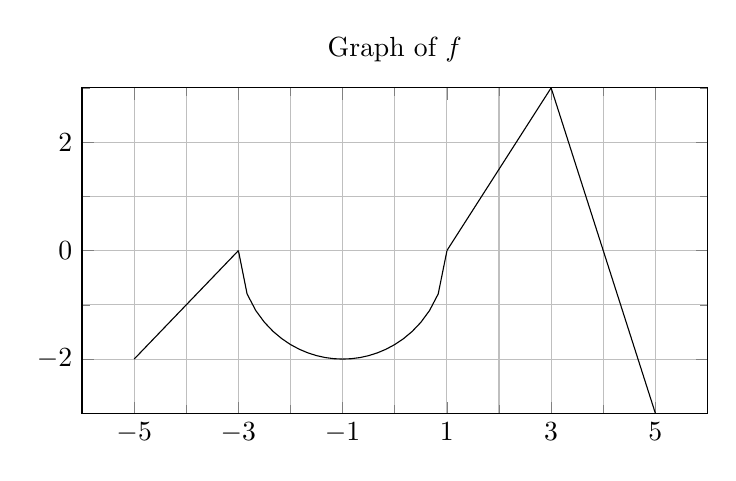
\begin{tikzpicture}
        \begin{axis}[cycle list=black, minor xtick={-5, -4, ..., 5},
          grid=minor, minor ytick={-4, -3, ..., 4}, ymin=-3, ymax=3,
          xtick={-5, -3, ..., 5}, width=3.75in, height=2.25in, title=Graph
          of $f$]
          \addplot+[domain=-5:-3] {x+3};
          \addplot+[domain=-3:1] {-sqrt(4-(x+1)^2)};
          \addplot+[domain=1:3] {1.5 * (x - 1)};
          \addplot+[domain=3:5] {-3*(x-4)};        
        \end{axis}
      \end{tikzpicture}
      }

    \begin{center}
      \usebox{\graph}
    \end{center}

    \begin{enumerate}
    \item \label{spring2004-spring2011-mb-final-combined-evaluate}
      Find each of the following values.  If a value is not defined,
      explain why not.

      \begin{enumerate}
      \item
        \begin{problem}[\vfill]
          $G(-3)$
        \end{problem}

        \begin{solution}
          By definition of $G$, $\displaystyle G(-3) = \int_{-3}^{-3}
          f(t)\,dt$, and this is $\boxed{0}$.
        \end{solution}

      \item
        \begin{problem}[\vfill]
          $G(-5)$
        \end{problem}

        \begin{solution}
          By definition of $G$, $\displaystyle G(-5) = \int_{-3}^{-5}
          f(t)\,dt$, and this is equal to $\displaystyle - \int_{-5}^{-3}
          f(t)\,dt = 2$.
        \end{solution}

      \item
        \begin{problem}[\vfill]
          $G(1)$
        \end{problem}

        \begin{solution}
          By definition of $G$, $\displaystyle G(1) = \int_{-3}^1
          f(t)\,dt$; from the graph, we can see that this is the negative
          of the area of a semi-circle of radius 2, or $- \frac{1}{2}
          \cdot \pi \cdot 2^2 = \boxed{-2\pi}$.
        \end{solution}

      \item
        \begin{problem}[\vfill]
          $G'(1)$ 
        \end{problem}

        \begin{solution}
          By FTOC 1, $G'(1) = f(1)$, which is $\boxed{0}$ (by looking at
          the graph of $f$).
        \end{solution}

      \item
        \begin{problem}[\vfill\newpage]
          $G''(1)$
        \end{problem}

        \begin{solution}
          By FTOC 1, this is $f'(1)$, and we can see from the graph of $f$
          that this is \fbox{undefined}.
        \end{solution}

      \end{enumerate}

    \end{enumerate}

    \continueproblem{\emph{Continued from previous page:} $\displaystyle
      G(x) = \int_{-3}^x f(t)\,dt$ where $f$ is the function whose graph
      is given below.
    \begin{center}
      \usebox{\graph}
      \end{center}
    }

    \begin{enumerate}[resume]

    \item
      \begin{problem}[\vfill]
        For what values of $x$ in $(-5, 5)$ is $G(x)$ decreasing?  Justify
        your answer.
      \end{problem}

      \begin{solution}
        Our usual strategy for such a question is to make a sign chart for
        $G'$.  By FTOC 1, $G' = f$, so we're really making a sign chart
        for $f$:
        \begin{center}
          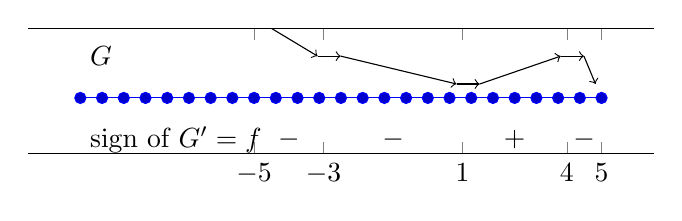
\begin{tikzpicture}
            \begin{axis}[axis y line=none, x axis line style={-}, xtick={-5., -3., 1., 4., 5.}, xticklabels={$-5$, $-3$, $1$, $4$, $5$}, ymin=-2, ymax=2.5, height=1.25in, width=3.75in]
              \addplot+[domain=-10.:5.]{0};
              \draw (axis cs: -10., -1.5) node[right] {sign of $G' = f$};
              \draw (axis cs: -10., 1.5) node[right] {$G$};
              \draw (axis cs: -4., -1.5) node{$-$};
              \draw[->, xshift=2pt] (axis cs: -4.66667, 2.5) -- (axis cs: -3.33333, 1.5);
              \draw (axis cs: -1., -1.5) node{$-$};
              \draw[->, xshift=2pt] (axis cs: -2.66667, 1.5) -- (axis cs: 0.666667, 0.5);
              \draw (axis cs: 2.5, -1.5) node{$+$};
              \draw[->, xshift=2pt] (axis cs: 1.33333, 0.5) -- (axis cs: 3.66667, 1.5);
              \draw (axis cs: 4.5, -1.5) node{$-$};
              \draw[->, xshift=2pt] (axis cs: 4.33333, 1.5) -- (axis cs: 4.66667, 0.5);
              \draw[->, xshift=2pt] (axis cs: -3.33333, 1.5) -- (axis cs: -2.66667, 1.5);
              \draw[->, xshift=2pt] (axis cs: 0.666667, 0.5) -- (axis cs: 1.33333, 0.5);
              \draw[->, xshift=2pt] (axis cs: 3.66667, 1.5) -- (axis cs: 4.33333, 1.5);
            \end{axis}
          \end{tikzpicture}
        \end{center}
        From this, we can see that $G$ is decreasing on \fbox{$(-5, 1)$ and
          $(4, 5)$}.  (It's also fine to say $G$ is decreasing on $(-5,
        -3)$, $(-3, 1)$, and $(4, 5)$.)
      \end{solution}

    \item % added
      \label{spring2004-spring2011-mb-final-combined-abs-min}
      \begin{problem}[\vfill]
        Does $G(x)$ have an absolute minimum value on $[-5, 5]$?  If so,
        what is this value and where (that is, at what $x$-value) does it
        occur?  Justify your answer.
      \end{problem}

      \begin{solution}
        Since $[-5, 5]$ is a closed interval and $G$ is continuous, $G$ must
        have an absolute maximum on $[-5, 5]$.  From our sign chart, we see
        that the absolute maximum must occur either at $1$ or $5$.  To
        decide which, let's evaluate $G(1)$ and $G(5)$:
        \begin{align*}
          G(1) &= - 2 \pi \text{ from
            \ref{spring2004-spring2011-mb-final-combined-evaluate}} \\
          G(5) &= \int_{-3}^5 f(t)\,dt = - 2 \pi + 3
        \end{align*}
        The smaller of these two is $G(1)$, so $G$ has an absolute minimum
        at $\boxed{x = 1}$, and the absolute minimum value is
        $\boxed{-2\pi}$.
      \end{solution}

    \item
      \begin{problem}[\vfill\newpage]
        Does $G(x)$ have an absolute maximum value on $[-5, 5]$?  If so,
        what is this value and where (that is, at what $x$-value) does it
        occur?  Justify your answer.
      \end{problem}

      \begin{solution}      
        Since $[-5, 5]$ is a closed interval and $G$ is continuous, $G$ must
        have an absolute maximum on $[-5, 5]$.  From our sign chart, we see
        that the absolute maximum must occur either at $-5$ or $4$.  To
        decide which, let's evaluate $G(-5)$ and $G(4)$.

        In \ref{spring2004-spring2011-mb-final-combined-evaluate}, we found
        that $G(-5) = 2$.  On the other hand, $G(4) = \displaystyle
        \int_{-3}^4 f(t)\,dt = - 2 \pi + \frac{9}{2}$; this is negative,
        so $G(-5)$ is greater.  Therefore, the absolute maximum of $G$
        occurs at $\boxed{x = -5}$, and the absolute maximum value is
        $G(-5) = \boxed{2}$.
      \end{solution}

    \end{enumerate}

    \continueproblem{\emph{Continued from previous page:} $\displaystyle
      G(x) = \int_{-3}^x f(t)\,dt$ where $f$ is the function whose graph
      is given below.
    \begin{center}
      \usebox{\graph}
      \end{center}
    }

    \begin{enumerate}[resume]
    \item
      \begin{problem}[\vfill]
        For what values of $x$ in $(-5, 5)$ is $G(x)$ concave down?  Justify 
        your answer.
      \end{problem}

      \begin{solution}
        $G$ is concave down when $G' = f$ is decreasing, which happens on
        \fbox{$(-3, -1)$ and $(3, 5)$}.
      \end{solution}

    \item
      \begin{problem}[\stretch{2}]
        Sketch the graph of $G(x)$ on $[-5, 5]$.  Clearly label any
        important values on the axes. 
      \end{problem}

      \begin{solution}
        \begin{center}
          \begin{tikzpicture}
            \begin{axis}[cycle list=black, xtick={-5, -3, ..., 5},
              ytick={-6.28, 2}, yticklabels={$-2\pi$, 2}]
              \addplot+[domain=3.:5]{0.5*(-51.56637061435917 + 24.*x - 3.*x^2)};
              \addplot+[domain=-5:-3.]{0.5*(9. + 6.*x + x^2)};
              \addplot+[domain=1.:3.]{0.25*(-22.132741228718345 - 6.*x + 3.*x^2)};
              \addplot+[domain=-3.:1.]{0.5*(-6.283185307179586 - 1.*sqrt(3. - 2.*x - 1.*x^2) - 1.*x*sqrt(3. - 2.*x - 1.*x^2) - 4/180*pi*asin(0.5*(1. + x)))};
            \end{axis}
          \end{tikzpicture}
        \end{center}
      \end{solution}

      \begin{grading}
        Key features of the graph:
        \begin{itemize}
        \item It passes through $(-3, 0)$.
        \item It should decrease on $(-5, 1)$, increase on $(1, 4)$, and
          decrease on $(4, 5)$.  It should also have a horizontal tangent
          line at $x = -3$.
        \item Its highest point is $(-5, 2)$, and its lowest point is $(1,
          -2\pi)$.
        \item It is concave up on $(-5, -3)$, concave down on $(-3, -1)$,
          concave up on $(-1, 3)$, and concave down on $(3, 5)$. 
        \end{itemize}
      \end{grading}

    \item Suppose that the function $f(t)$ above represents the rate of
      change of the population of a small town, in people per day, where $t$
      is measured in days and $t = 0$ is February 15, 2012.  On February 16,
      the town has a population of 1000.

      \begin{enumerate}

      \item
        \begin{problem}[\stretch{0.5}]
          What quantity is represented by $G(4)$?  Your answer should be in
          terms of population and dates in February. 
        \end{problem}

        \begin{solution}
          $G(4) = \displaystyle \int_{-3}^4 f(t)\,dt$ is the net change in
          population between February 12 ($t = -3$) and February 19 ($t =
          4$).
        \end{solution}

      \item
        \begin{problem}[\vfill\newpage]
          What is the town's population on February 18?  (Please simplify
          your answer; it should not involve any integral signs.)
        \end{problem}

        \begin{solution}
          We are told that, on February 16 ($t = 1$), the town has a
          population of 1000 people.  The net change from February 16 ($t =
          1$) to February 18 ($t = 3$) is $\displaystyle \int_1^3 f(t)\,dt$,
          so the total population on February 18 is $\displaystyle 1000 +
          \int_{1}^3 f(t)\,dt = 1000 + 3 = \boxed{1003}$ people.
        \end{solution}

      \end{enumerate}

    \end{enumerate}
  }

    \pspace{\newpage}
\item 


  \label{spring2010-mb-final-9-parts} 

  \textbf{Multiple choice.} The parts below are unrelated; no justification
  is needed.  

  \begin{enumerate}

  \item Suppose that $f(x)$ is a continuous function and $a$ and $b$ are
    real numbers. Circle all choices that complete the statement correctly.
    \begin{center}
      The derivative with respect to $x$ of $\displaystyle \int_a^b
      f(x)\,dx$ is \fitb{1in}{}.
    \end{center}


      \begin{enumerate}[label=\protect\maybecircle{\Alph*.}]
      \plainitem $f(x)$
      \circleitem 0
      \plainitem $f(b)$
      \plainitem None of the above.
      \end{enumerate}
      \pspace{\vfill}

    \begin{solution}
      $\displaystyle \int_a^b f(x)\,dx$ is a constant, so the derivative of
      $\displaystyle \int_a^b f(x)\,dx$ is zero.  (It may help to make this
      more concrete by thinking of specific numbers, like $a = 1, b = 3$.)      
    \end{solution}

  \item 

    Suppose that $f(x)$ is a positive continuous function with $f(0) = 7$.
    Let $F(x) = \displaystyle \int_0^x f(t)\,dt$ and $G(x) = \displaystyle
    \int_2^x f(t)\,dt$.  Decide whether the following statements are
    definitely true or definitely false, or if there is not enough
    information to be sure.  Please circle your choice.

    \providecommand{\answerblock}{}
    \renewcommand{\answerblock}[1]{%
      \hfill \solonly{\maybecircle[#1=1]}{True} \quad
      \solonly{\maybecircle[#1=2]}{False} \quad
      \solonly{\maybecircle[#1=3]}{Not enough info}
    }

    \begin{enumerate}
    \item
      \begin{problem}
        $F'(x) = G'(x)$. \answerblock{1}
      \end{problem}

      \begin{solution}
        By FTOC 1, $F'(x)$ and $G'(x)$ are both equal to $f(x)$.
      \end{solution}

    \item
      \begin{problem}
        $F(0) = 7$. \answerblock{2}
      \end{problem}

      \begin{solution}
        $F(0)$ is defined to be $\displaystyle \int_0^0 f(t)\,dt$, which
        is 0.
      \end{solution}

    \item
      \begin{problem}
        $G(0) = 7$. \answerblock{2}
      \end{problem}

      \begin{solution}
        $G(0)$ is defined to be $\displaystyle \int_2^0 f(t)\,dt$, which
        must be negative because $f$ is a positive function. 
      \end{solution}

    \item
      \begin{problem}
        \parbox[t]{3in}{The graphs of $F(x)$ and $G(x)$ are vertical
          shifts of each other.} \answerblock{1}
      \end{problem}

      \begin{solution}
        We've already seen that $F' = G'$, and two continuous functions
        with the same derivative must be vertical shifts of each other.
        (Alternatively, we can use properties of integrals to verify that
        $F(x) - G(x) = \displaystyle \int_0^2 f(t)\,dt$, which is a
        constant.)
      \end{solution}

    \end{enumerate}
    \pspace{\vfill}

\end{enumerate}
\end{enumerate}
\end{document}

